\documentclass{article}
\usepackage{tikz}
\usetikzlibrary{arrows,shapes,positioning,shadows,trees}

\usepackage[paperwidth=25cm,paperheight=22cm,left=1cm,top=1cm]{geometry}
\tikzset{
  basic/.style  = {draw, text width=2cm, drop shadow, font=\sffamily, rectangle},
  root/.style   = {basic, rounded corners=2pt, thin, align=center,
                   fill=green!30},
  level 2/.style = {basic, rounded corners=6pt, thin,align=center, fill=green!60,
                   text width=8em},
  level 3/.style = {basic, thin, align=left, fill=pink!60, text width=6.5em}
}

\begin{document}
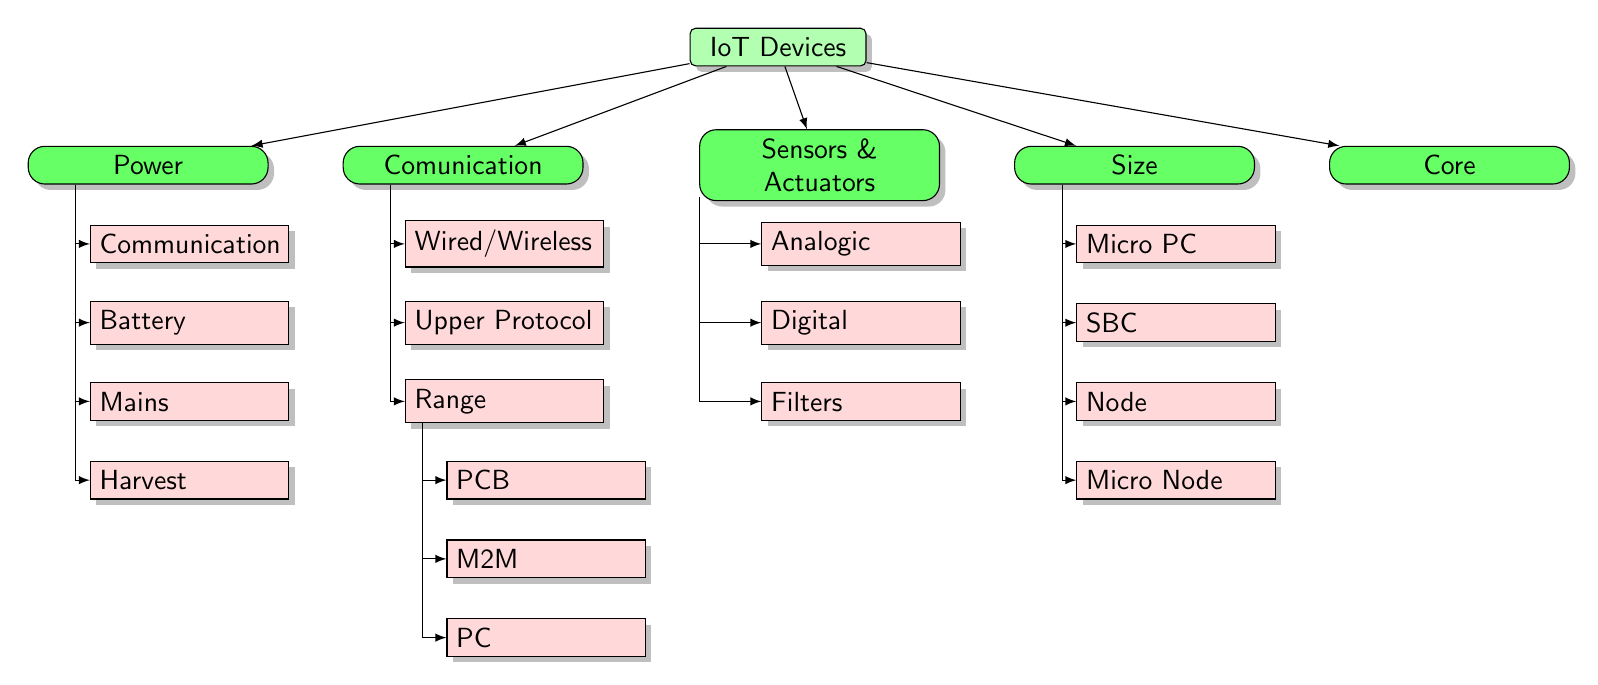
\begin{tikzpicture}[
  level 1/.style={sibling distance=40mm},
  edge from parent/.style={->,draw},
  >=latex]

% root of the the initial tree, level 1
\node[root] {IoT Devices}
% The first level, as children of the initial tree
  child {node[level 2] (c1) {Power}}
  child {node[level 2] (c2) {Comunication}}
  child {node[level 2, xshift=15pt] (c3) {Sensors \& Actuators}}
  child {node[level 2, xshift=15pt] (c4) {Size}}
  child {node[level 2, xshift=15pt] (c5) {Core}};

%Power
\begin{scope}[every node/.style={level 3}]
\node [below of = c1, xshift=15pt] (c11) {Communication};
\node [below of = c11] (c12) {Battery};
\node [below of = c12] (c13) {Mains};
\node [below of = c13] (c14) {Harvest};

%Communication
\node [below of = c2, xshift=15pt] (c21) {Wired/Wireless};
\node [below of = c21] (c22) {Upper Protocol};
\node [below of = c22] (c23) {Range};
  \node[below of = c23, xshift=15pt](c231){PCB};
  \node[below of = c231](c232){M2M};
  \node[below of = c232](c233){PC};
%Sensor & actuators
\node [below of = c3, xshift=15pt] (c31) {Analogic};
\node [below of = c31] (c32) {Digital};
\node [below of = c32] (c33) {Filters};

%Size
\node [below of = c4, xshift=15pt] (c41) {Micro PC};
\node [below of = c41] (c42) {SBC};
\node [below of = c42] (c43) {Node};
\node [below of = c43] (c44) {Micro Node};

\end{scope}
% lines from each level 1 node to every one of its "children"
\foreach \value in {1,...,4}
  \draw[->] (c1.195) |- (c1\value.west);

\foreach \value in {1,...,3}
  \draw[->] (c2.195) |- (c2\value.west);
\foreach \value in {1,...,3}
 \draw[->] (c23.195) |- (c23\value.west);

\foreach \value in {1,...,3}
  \draw[->] (c3.195) |- (c3\value.west);
  
\foreach \value in {1,...,4}
  \draw[->] (c4.195) |- (c4\value.west);
\end{tikzpicture}
\end{document}
